\documentclass{article}
\usepackage[margin=0.5cm]{geometry}
\usepackage{tikz}
\begin{document}

\usetikzlibrary {folding}
\begin{tikzpicture}[scale=10]
  \pic [
    folding line length=6mm,
    transform shape,
    face 1= { \node[text width=2.9cm,text height=11pt,scale=0.2,inner sep=10pt] {

        {\bf Cayendo en las redes de Venecia}\\
        ~\\
        JJ Merelo};
    },
    face 2= { \node{ Tibi }; },
    face 3= { \node{\tiny Marce}; },
    face 4= { \node{\tiny Evangelista}; },
    face 5= { \node{\tiny Meus}; },
    face 6= {  \node[anchor=center] {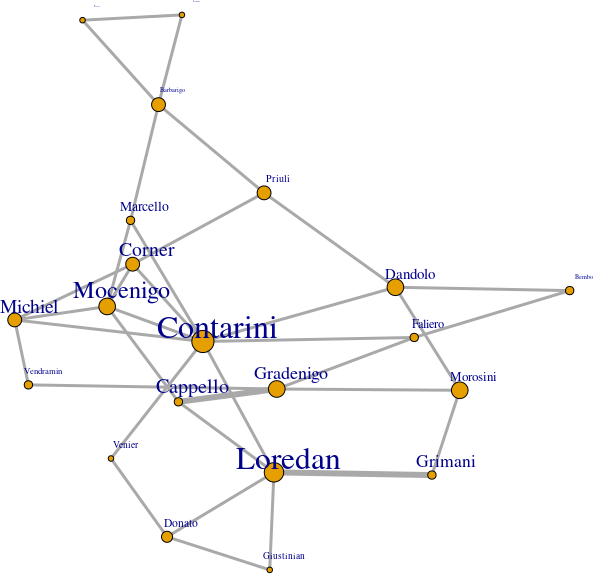
\includegraphics[width=0.6cm]{dogos} };}
  ]
  { cube folding };
\end{tikzpicture}

\end{document}